\section{Introduction} % Approx word count = 1000 words (total = 1250)

% Al26 Intro & Observations
Aluminium-26 ($^{26}$Al) is a relatively long-lived, radioactive isotope with a half life of $\lambda = 0.72$ Myrs \citep{Iliadis2015}.
It is observed in the Galaxy via $\gamma$-ray spectroscopy of its 1.81 MeV decay to $^{26}$Mg \citep{2004ESASP.552...27D}.
An excess of $^{26}$Mg has been found in meteorite samples \citep{1978ApJ...224L.139A} and pre-solar grains \citep{2011ApJS..193...16I}, indicating that more $^{26}$Al was present in the early solar system than the current galactic average \citep[see][]{2019ApJ...884...38B}.
\cite{2011ApJS..193...16I} note that ``the observation of Galactic $\gamma$-rays from $^{26}$Al is important since it provides unambiguous direct evidence for ... nucleosynthesis in stars'' even if ``the origin of $^{26}$Al remains controversial''.

\subsection{Aluminium-26 Production in Stars}

% Stellar evolution
% Stars are created in galaxies from material in the interstellar medium (ISM). Nuclear reactions in stars alters the composition of this material as they evolve. Ultimately, when a star dies, this material is returned to the ISM and goes on to create new generations of stars. The resulting evolution of chemical composition in galaxies is called galactic chemical evolution (GCE).
% Stellar nucleosynthesis is responsible for creating almost all elements beyond hydrogen and helium\footnote{Excepting man-made elements and elements formed in the ISM by cosmic ray spallation.} and also keeps stars stable during their lifetimes: energy released from fusion generates an outward thermal pressure that comes into hydrostatic equilibrium with the inwards pressure of the star's own weight.

Stars spend most of their lives on the main sequence, generating energy from hydrostatic fusion of $^1$H into $^4$He in the core.
Hydrogen-burning reactions range from the simple proton-proton chains dominant in low mass stars, to cycles of proton-capture and $\alpha$-decay reactions that use heavier elements as catalysts such as the CNO cycle dominant in high mass stars \citep{Iliadis2015}.

After exhausting hydrogen in the core, the stellar envelope cools and expands as the core contracts and heats up. Meanwhile, hydrogen-burning continues in a shell layer around the core.
With sufficient mass, stellar cores can reach temperatures high enough to fuse heavier elements, the first of which is helium.
Depending on their initial mass, stars can burn through carbon, neon, oxygen, and ultimately silicon.
Massive stars end their lives in core collapse supernovae (CCSN), leaving behind a neutron star or a black hole \citep{Carroll2007}.

\begin{figure}
    \centering
    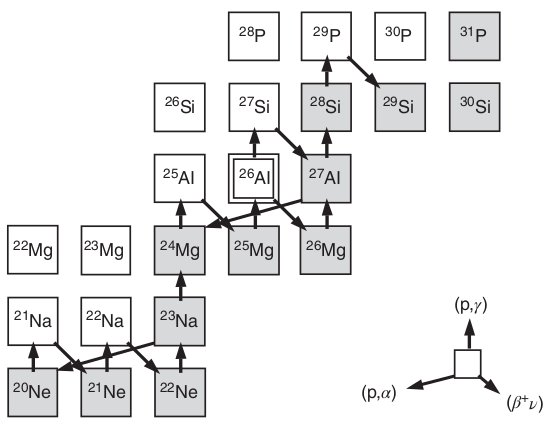
\includegraphics[width=\columnwidth]{figures/intro/AlMg.png}
    \captionsetup{width=0.9\columnwidth}
    \caption{The hydrogen-burning neon-sodium (Ne-Na) \& aluminium-magnesium (Al-Mg) cycles represented on the chart of nuclides.
    The orientation of each arrow represents a particular reaction: proton capture ($\mathrm{p,\gamma}$), $\mathrm{\beta^+}$ decay ($\mathrm{\beta^+\nu}$), and helium emission ($\mathrm{p,\alpha}$).
    Diagram from \cite{Iliadis2015}.}
    \label{fig:reactions}
\end{figure}

% Al26 Production and Destruction
In massive stars, $^{26}$Al is created in both core and shell hydrogen burning via the Al-Mg cycle (see figure \ref{fig:reactions}): a catalytic series of reactions similar to the CNO cycle.
In the absence of production channels, $^{26}$Al decays to $^{26}$Mg during helium-burning and is also destroyed via neutron capture reactions \citep{2019ApJ...884...38B}.
It is later produced in carbon and neon-burning convective shells \citep{1978ApJ...224L.139A} and ejected in the supernova, which synthesises additional $^{26}$Al via explosive neon-burning \citep{2006ApJ...647..483L}.
These latter sources are by far the largest contributor to stellar $^{26}$Al yields\footnote{A star's isotope `yield' is defined as the mass of that isotope ejected from the star over its lifetime. Pre-supernova yields can be calculated by integrating the surface abundance of the isotope multiplied by the surface mass-loss rate with respect to time.}.

% Al26 isomer
$^{26}$Al can be formed either in its ground state $^{26}$Al$^g$ or an isomeric\footnotemark state $^{26}$Al$^m$.
While most isotopes come into thermal equilibrium with their excited states, $^{26}$Al represents a rare exception and does not reach equilibrium below T = 0.4 GK \citep{Iliadis2015}. Thus each state is considered individually during the hydrogen-burning stage. 
\footnotetext{An isomeric state is a relatively long lived excited state with a half life on the order of seconds to days.}
In this paper, $^{26}$Al is used to refer exclusively to $^{26}$Al$^g$; we are not concerned with $^{26}$Al$^m$ since it decays too quickly for it to contribute meaningfully to $^{26}$Al yields.

% Ejecting Al26 with winds
Stellar winds eject material from the surface into the interstellar medium (ISM).
Main sequence winds are not usually strong enough to extract much $^{26}$Al, but helium-burning winds can eject $^{26}$Al produced in shell hydrogen burning layers and in some cases much of the $^{26}$Al left over from the main sequence.
Stars with initial mass greater than ~20 M$_{\sun}$ regularly eject their entire envelopes and hydrogen-burning shells, becoming a Wolf-Rayet (WR) star \citep{Carroll2007}.

% Ejecting Al26 with RLOF
Another way in which stars eject material is through mass transfer with a binary companion.
Since $^{26}$Al is created during hydrogen-burning and destroyed during helium-burning, mass transfer must occur between zero-age main sequence (ZAMS) and the end of helium-burning in order to contribute significantly to $^{26}$Al yield.

\subsection{Aluminium-26 from Binary Stars}

\begin{figure}
    \centering
    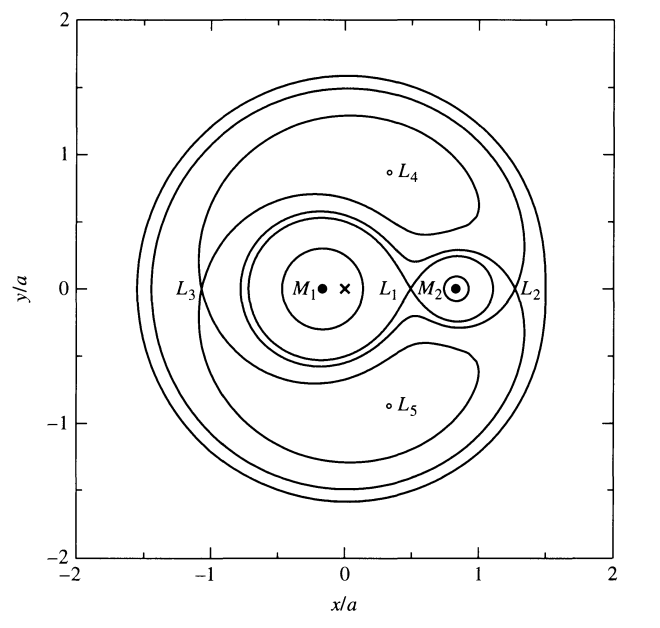
\includegraphics[width=\columnwidth]{figures/intro/RL.png}
    \captionsetup{width=0.9\columnwidth}
    \caption{Equipotential lines around a binary system consisting of stars M$_1$ and M$_2$. The $\times$ marks the centre of mass, while L$_1$ is the zero-potential inner-Lagrangian point between both stars. Note that the equipotential lines passing through this point define the Roche lobes of each star.
    Diagram from \cite{Carroll2007}}
    \label{fig:RocheLobes}
\end{figure}

A binary system consists of two stars orbiting their centre of mass.
Their mean separation can vary greatly, with distant binaries experiencing little to no interaction.
Tidal effects in close binaries bring the stars closer together \citep[see][]{Iliadis2015}, increasing the likelihood of mass transfer, or even common envelope evolution\footnote{Common envelope evolution occurs when binary stars are close enough to physically overlap.}.
There is still uncertainty as to what proportion of stars exist as part of an interacting binary system.
However, \cite{2012Sci...337..444S} found that binary interactions are the norm for massive stars, with over 70\% experiencing mass transfer at some point in their evolution.

There are two processes responsible for binary mass transfer: stellar winds\footnote{The effects of wind mass transfer are minimal compared to RLOF, as only a very small fraction of mass lost by stellar winds is accreted onto the companion.} and Roche lobe overflow (RLOF).
The latter occurs when a star in a binary system, usually the primary\footnote{Since the first major expansion in stellar radius occurs after the main-sequence and more massive stars evolve faster than lower mass stars, it is more likely for the more massive primary to enter RLOF before the secondary.}, expands beyond the central zero-potential point $L_1$\footnote{$L_1$ is called the inner Lagrangian point and is situated at a point between the stars where the gravitational potential of both stars cancels to zero. There are also four outer Lagrangian points ($L_2$ through $L_5$) in a binary system.}.
Figure \ref{fig:RocheLobes} depicts the gravitational equipotential surfaces around binary stars; such surfaces are spherical around a single star, but in binaries they are deformed towards $L_1$ to form teardrop-shaped Roche lobes which together define a three-dimensional figure-8 \citep{Iliadis2015}.

When a star fills its Roche lobe, material is stripped from the surface, through $L_1$, and into the Roche lobe of its companion.
From here, the lost material is either accreted onto the companion or ejected into the ISM.
The fraction of the mass lost that is accreted onto the companion is called the mass transfer efficiency $\beta$\footnotemark, ranging from $\beta = 1$ (fully conservative) to $\beta = 0$ (fully non-conservative).
\footnotetext{In this paper, $\beta$ is used to denote the fraction of the mass lost from the mass-losing star that is accreted onto the partner star during RLOF. Please note that other documents, including \cite{2019ApJ...884...38B}, use $1 - \beta$ to mean the same thing.}
Mass transfer through RLOF is further classified based on the evolutionary stage of the mass-losing star: case A for the main-sequence, C for helium-burning, and B for the Hertzsprung gap between these stages.

\subsection{Aims of This Study}

This study investigates the effects of mass transfer on the $^{26}$Al production of massive binary stars compared to their single star counterparts.
$^{26}$Al production in massive binaries was recently studied by \cite{2019ApJ...884...38B} who found that the effects of binary interaction can differ dramatically depending on various parameters.
%
Here, we investigate the effects of the initial masses, orbital period, and mass transfer efficiency.
While the focus is on $^{26}$Al, the processes observed in these simulations may be of use for binary studies for any isotope.
We also aim to demonstrate the potential for binary phenomena to impact stellar nucleosynthesis and to stress the role of binaries in galactic chemical evolution.